\documentclass[12pt,conference]{IEEEtran}
\usepackage{mathtools}

\usepackage{algorithm}% http://ctan.org/pkg/algorithms
\usepackage{algpseudocode}% http://ctan.org/pkg/algorithmicx

\usepackage{graphicx}
\usepackage{amsmath}

\usepackage{stfloats}

\DeclareMathOperator{\atantwo}{atan2}
\graphicspath{ {images/} }

\hyphenation{op-tical net-works semi-conduc-tor}

\begin{document}
\raggedbottom

\title{Improving the Accuracy of a Sequential Mining Model for Hurricane Trajectory Prediction}

\author{\IEEEauthorblockN{Taylor Cox, Caden Marofke}
\IEEEauthorblockA{Department of Computer Science\\
University of Manitoba\\
Winnipeg, Manitoba\\
Email: \{coxt3, marofkec\}@myumanitoba.ca}}

\maketitle
% Clearly state that weighted support is our idea, inspired by some work but we have a diff approach
\begin{abstract}

In the 21st century alone, hurricanes have caused billions of dollars worth of damage due to property destruction, personal danger, and civil unrest. The catastrophic impact of hurricanes and other tropical storms has motivated extensive research into hurricane forecasting. Hurricane trajectory prediction is a subfield of hurricane forecasting that traditionally uses meteorological analysis to determine the future path of a given hurricane. While meteorological methods of hurricane trajectory prediction have been effective in the past, little attention has been paid to hurricane trajectory prediction with respect to historical frequent pattern mining. In this work, we present multiple dimensions for improving the accuracy of data mining-based hurricane trajectory prediction. We first propose the use of the Haversine distance formula for realistic hurricane trajectory distance comparison. We also introduce the use of weighted training data to favour recent hurricane trends when determining a trajectory prediction. Finally, we use training data exclusively from the years 1950 to 2000 to reduce the impact of historical climate trends and inaccuracies in hurricane recording methodologies. After implementing all three improvement dimensions on a contemporary data mining model for hurricane trajectory prediction based on AprioriAll, results show a prediction-correctness ratio up to 10.0\% higher than the current state-of-the-art, at 75.0\%.

\end{abstract}

\begin{IEEEkeywords}
Hurricane Trajectory, AprioriAll, Prediction, Pattern Matching
\end{IEEEkeywords}

\IEEEpeerreviewmaketitle

\section{Introduction}

Hurricanes are a specific type of tropical cyclone exclusive to the Atlantic basin. Hurricanes are divided into five categories according the Saffir-Simpson scale, based on wind-speed and expected damage. In the United States alone, the damages incurred by a single hurricane have reached as high \$157BN \cite{hurricane-cost}. The damages incurred by hurricanes do not only include property damage, but also personal danger and in some cases widespread civil unrest \cite{hurricane-cost-non-financial}. These damages motivate extensive research in the field of hurricane prediction analysis. Hurricane prediction analysis is traditionally divided into the subfields of hurricane intensity prediction and hurricane trajectory prediction. This paper focuses exclusively on the subfield of hurricane trajectory prediction. In particular, the goal of this paper is to investigate and refine the existing-state-of-the art in hurricane trajectory prediction systems based on sequential data mining.

Data mining is the nontrivial extraction of implicit, previously unknown, and potentially useful information from data \cite{data mining-def}. Data mining applies to an extremely wide range of applications, including clickstream mining, social network community detection, and artificial intelligence. The data mining sub-discipline of particular interest in this work is \textit{sequential} data mining. Sequential data mining uses a database of chronologically ordered inputs to mine frequent patterns and interesting association rules. These association rules are used to make predictions on future data entries such as future customer transactions. More specifically, association rules generated by sequential data mining algorithms including AprioriAll, SPIRIT and PrefixSpan can be used as training data for a hurricane trajectory prediction model.

The existing standard in hurricane trajectory prediction via association rule mining is established by Dong et al in \cite{major-hurricane-model}. The work cited proposes a hurricane trajectory prediction model based on data mining (HTPDM) that uses a modified variant of AprioriAll, a standard algorithm for mining sequential data \cite{AprioriAll-original}. HTPDM executes AprioriAll against historical hurricane trajectories from 1900 to 2000 to generate interesting trajectory association rules. These association rules are compared against test data composed of hurricane trajectories from 2001 to 2008. HTPDM divides a given testing trajectory into two parts: the initial trajectory $T_{i}$ and the terminal trajectory $T_{t}$. $T_{i}$ is compared against all association rule antecedents until a sufficiently matching rule R is found based on a predetermined fitness function. The consequent of R is then compared against $T_{t}$ using pattern-matching techniques to determine if the prediction was correct. The results of HTPM showed that the model was able to achieve a best-case correctness ratio of 65.0\%. In this work, a model similar to HTPDM will be implemented and various strategies will be employed to increase the correctness ratio. Reducing the impact of historical factors, favouring the impact of recent trends, and improving the realism of the hurricane trajectory prediction model result in a new model dubbed WARD-HTP (Weighted-Asset, Realistic-Distance Hurricane Trajectory Predictor). The strategies employed in WARD-HTP ultimately result in a correctness ratio of 75.0\%, a 10\% improvement over HTPDM.

The remainder of this paper is structured as follows: First, Section II gives a detailed survey of related work in the hurricane prediction and sequential mining disciplines. Next, section III will cover the general motivations of this work with respect to hurricane trajectory prediction and the specific motivations of this work with respect to improving the current state-of-the-art. Section IV will provide a description of the problem space, which includes specific implementation considerations in hurricane trajectory prediction. Section V will give an exposition of the solutions proposed in WARD-HTP for increasing the correctness ratio in hurricane trajectory prediction. Following that, Section VI will detail the experimental setup, including the training data and other experimental variables. Section VII will evaluate the results of the experiments, which show that the ideal configurations of WARD-HTP result in a maximal correctness ratio of 75.0\%. Finally, section VIII will capture all conclusions and proposed directions for future work.

\section{Related Work}

The development of an accurate hurricane trajectory prediction model is a problem which has received little attention in the data mining literature. Works including \cite{hurricane-intensity-1} and \cite{hurricane-intensity-2} have been completed to develop data-mining approaches to hurricane intensity prediction. These works however do not describe approaches to hurricane trajectory prediction. Hurricane trajectory prediction has been covered in previous meteorological and geographic information system (GIS) works. These types of hurricane trajectory forecasting models include those seen in \cite{hurricane-forecasting-1} or \cite{hurricane-forecasting-2}. The intersection between data mining and hurricane trajectory prediction has been sparsely investigated in the literature. Publications such as \cite{typhoon-clustering} proposed a clustering-based model for typhoon track prediction based on specific characteristics of historical data. Typhoons are then clustered into groups depending on the general trajectory patterns they exhibit. While the described work provided novel results in typhoon track clustering, it is not clear if the proposed solution is able to predict the trajectories of new storms. Additionally, the clusters developed apply specifically to typhoons, which are tropical storms native to the east-pacific seaboard. Such storm patterns may not be applicable to patterns found in hurricanes, which are exclusive to the Atlantic basin. For these reasons, the proposed clustering patterns were not used in this work.

The primary baseline of this work is \cite{major-hurricane-model}, which uses a specific implementation of AprioriAll (first proposed in \cite{AprioriAll-original}) to determine frequent hurricane trajectory patterns. These trajectory patterns correspond to interesting trajectory association rules, which are used to train a prediction model. The implementation of AprioriAll used in \cite{major-hurricane-model} also serves as the foundation for the model proposed in this work. AprioriAll transforms a transaction database into a \textit{customer} database, where each entry contains a customer and an ordered sequence of purchased items. The ordered sequence database is then mined for frequent ordered sequences.

The model proposed in this work uses historical hurricane trajectory readings from HURDAT2, the canonical hurricane database maintained by the National Hurricane Center \cite{HURDAT2-original}. The data in HURDAT2 was sorted into $\langle Hurricane, Trajectory \rangle$ pairs, removing the need for the sequence mapping step required at initialization of AprioriAll. The Atlantic hurricane trajectories recorded in HURDAT2 span a very large area, some of which reaching over 10,000 kilometres between the first and last recorded points. As a result, the coordinates recorded are limited to those within a range of 0 to 50 degrees north, and 20 to 100 degrees west. This degree range is approximately the size of the south Atlantic basin.

\section{Motivation}

There are two categories of motivation behind this work. The first motivation of this work is to add to the total investigation completed in the data mining-based hurricane trajectory prediction sub-discipline. Little research effort has been allocated to this particular problem space of high economic and social impact. This work is expected to contribute to the growing effort by academic and government researchers to develop reliable methods of hurricane trajectory prediction in the interest of public safety and economic stability.

The second motivation behind this work is the specific goal of improving the correctness ratio in the current standard data mining model for hurricane trajectory prediction. As previously described, HTPDM achieved a best case trajectory prediction correctness ratio of 65.0\%. This means that of all testing trajectory for which a matching rule was successfully produced, 65.0\% of such matches were correct predictions. When HTPDM accounted for testing trajectories with which no rule could be matched, the correctness ratio decreased by 7.5\% to a worst-case value of 57.5\% correctness. This decrease in accuracy is expected as some hurricane trajectories are outliers which cannot be predicted by frequent pattern mining, as will be discussed further in this work.

The motivation of improving the correctness ratio in the model encompasses the challenges of improving the best-case correctness ratio (the correctness ratio when ignoring rule-miss incidents) and the worst-case correctness ratio (the correctness ratio when accounting for rule-miss incidents). To fulfill the motivations of this work, a series of improvement strategies are proposed for the current standard hurricane trajectory prediction model based on AprioriAll. In general, these strategies seek to improve the realism of the prediction model, reduce historical factors which may negatively affect the model's correctness ratio, and favour recent hurricane trajectory trends which are likely to be reflected in current and future hurricane patterns.

\section{Problem Description}

In this section, the problems surrounding the achievement of accurate hurricane trajectory prediction are explained in detail. These problems consist of multiple challenges which apply generally to sequential data mining and specifically to hurricane distance, trajectory and location analysis. Many of the domain-specific challenges of hurricane trajectory prediction arise from the fact that hurricane points are tracked as a series of $\langle Latitude, Longitude \rangle$ points, which do \textit{not} directly correspond to traditional (x, y) coordinates, as latitude and longitude coordinates are points imposed upon a sphere. Challenges such as accurate distance evaluation are the result of the need to transition from a Euclidean to a Polar coordinate system.

The exposition of the hurricane prediction problem domain is divided into three parts. The first aspect of the problem domain concerns the underlying sequential mining approach used. This includes a thorough description of AprioriAll, its intended usage, and the reaction of AprioriAll to its input parameters. Next, the subproblem of region discretization will be discussed. Since $\langle Latitude, Longitude \rangle$ points describe continuous space, hurricane trajectories are converted to sequences of discrete regions to enable the discovery of frequent patterns. Finally, problems involving hurricane trajectory matching will be discussed. These problems include pattern matching for determining best fit rules and pattern matching for determining trajectory prediction correctness.

\subsection{AprioriAll}

In HTPDM and WARD-HTP, the algorithm that generates trajectory prediction possibilities is based on AprioriAll. AprioriAll was first proposed at IBM research as a method for discovering frequent sequential patterns in transactional databases \cite{AprioriAll-original}. In its original implementation, AprioriAll is able to generate association rules describing sentences of the form ``Customers who buy P may later buy Q''. In the hurricane trajectory prediction problem, AprioriAll is used to generate association rules describing sentences of the form ``Hurricanes located at P may later be located at Q''. In the context of AprioriAll, hurricanes are considered $customers$ and their sequences of recorded points are considered $transactions$. Consider the high-level implementation steps of AprioriAll as follows:

\begin{enumerate}
\item Map the transaction database into a customer database.
\item Generate frequent sequences based on minimum support.
\item Generate association rules based on minimum confidence.
\end{enumerate}

\subsubsection{Mapping}

In step (1) of AprioriAll, a given transaction database \textit{D} is grouped by its customers, and the frequent items purchased by customers in individual transactions are recorded in a temporary table. The contents of this temporary table are mapped to corresponding sequences to enable the mining of frequent transaction sequences from the original database. The intention of step (1) is to map \textit{D} in its original $\langle TransactionID, CustomerID, Items\rangle$ database form into a database \textit{D'} of the form $\langle CustomerID, ItemSequence\rangle$. 

The hurricane trajectory model in this work does not implement step (1), as the training data from HURDAT2 was instead translated into a $\langle HurricaneID, CoordinateSequence\rangle$ database as a preprocessing step before any aspects of the model are executed. Figure (1) shows an example of how the trajectory database is structured after the initial mapping stage. Only two dimensions are needed in the database, being the hurricane ID and the sequence of latitude-longitude coordinates. All hurricanes in HURDAT2 have an ID corresponding to the location (i.e. the Atlantic), the index ordered by appearance in the hurricane year, and the year itself. For example, hurricane Katrina of year 2005 corresponds to AL122005. By directly translating the data instead of processing it with AprioriAll, all trajectories in the original database are preserved. This includes coordinate sequences which may ultimately be infrequent. The sequential mapping of AprioriAll is performed as a preprocessing step so that the database used in the prediction model will always consist of hurricanes and their coordinate sequences. The prepared (mapped) database may therefore be mined directly without the need for repeated mapping in subsequent executions of AprioriAll.

\begin{figure}[ht]
\caption{Sample of mapped Hurricane-Coordinates database}
\centering
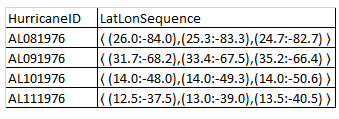
\includegraphics[scale=1.0]{hurricane-table-sample}
\end{figure}

\subsubsection{Sequence Generation}

Section (2) of AprioriAll is responsible for the generation of frequent sequences. In the case of hurricane trajectory prediction, these sequences correspond to frequently recorded hurricane coordinate sequences. Frequent hurricane coordinate sequences are those which occur at least a minimum number of times, as defined by the \textit{minimum support}, or minsup. In general terms, the sequence generation step of AprioriAll develops frequent ordered patterns of increasing length, beginning with frequent single-item sequences (corresponding to frequent single-point sequences). This step begins by scanning the $\langle HurricaneID, CoordinateSequence\rangle$ database for frequent single-point sequences. The frequent single-point trajectories are then converted to candidate two-point trajectories as the result of an inner join. The candidate two-point trajectories are scanned against the database to determine which candidates satisfy the minimum support. Another inner join generates the candidate 3-length trajectories. Once the sequence generation level reaches three, each candidate sequence must be pruned if any of their candidate subsequences are infrequent. Continuous execution of AprioriAll until termination results in the collection of all frequent hurricane trajectory patterns defined by the minimum support.

%AprioriAll Pseudocode
\begin{algorithm}[H]
  \caption{Modified AprioriAll: No Mapping Phase}
  \label{aprioriall_for_hurricanes}
  \begin{algorithmic}[1]
  \State{$L_{1} \gets \{Frequent\ Single\ Points\}$}
  \For{($k=2; L_{k-1} \neq \emptyset; k++)$}
    \State{$C_{k} \gets Candidates\ from\ Inner\ Join$}
    \State{$Prune\ C_{k}\ of\ infrequent\ subsequences\ $}
    \For{$sequence\ S \in HurricaneDB$}
      \State{$Increment\ c \in C_{k}\ support\ if\ c \in S$}
    \EndFor
    \State{$L_{k} \gets \{c \in C_{k}|\ sup(c) \geq minsup\}$}
  \EndFor
  \State{$Frequent Trajectories \gets All(L_{k})$}
  \end{algorithmic}
\end{algorithm}

As also seen in HTPDM, WARD-HTP executes AprioriAll with a slight modification to the existing algorithm proposed in \cite{AprioriAll-original}. Whereas L1 (the set of frequent single-item sequences) is generated by the L-Itemset (mapping) phase of AprioriAll, the variant of AprioriAll used in hurricane trajectory prediction skips the L-Itemset phase and thus scans the $\langle HurricaneID, CoordinateSequence\rangle$ database directly for frequent single-point trajectories. Otherwise, the remainder of AprioriAll is used in this work as originally designed. AprioriAll is used to ensure that the order of recorded hurricane coordinate sequences is preserved. This is a product of the inner-join step. Consider two hurricane trajectories $T_{1}$ and $T_{2}$. $T_{1}$ and $T_{2}$ form a new trajectory $T_{3}$ if and only if the \textit{L}-1 terminal coordinates of $T_{1}$ correspond to the \textit{L}-1 initial coordinates of $T_{2}$, where \textit{L} is the current level of AprioriAll being executed. For example, if \textit{L}$=$2, then AprioriAll scans for frequent 2-coordinate sequences, and uses those frequent 2-coordinate sequences to generate 3-coordinate sequences based on trajectory matching. If the matching condition is satisfied, a new trajectory is generated. The inner-join step of AprioriAll emulates the required hurricane trajectory-matching to discover frequent hurricane trajectory patterns. Once all possible frequent hurricane trajectory patterns are discovered, the second step of AprioriAll completes.

\subsubsection{Rule Generation}

The third and final step of AprioriAll is the rule-generation step. Though association rule generation is not a specific stage of the AprioriAll algorithm, it is traditionally the final stage of any association rule mining approach. The rule generation step is responsible for identifying and recording interesting association rules. As mentioned, rules generated by the hurricane trajectory prediction model proposed will satisfy sentences of the form ``Hurricanes located at P may later be located at Q''. 

Association rules are derived directly from frequent patterns generated by AprioriAll or any modified versions. These rules consist of four dimensions: the antecedent, consequent, support and confidence. An association rule \textit{R} is generated by partitioning a frequent sequence \textit{S} into two congruent parts. The left partition of \textit{S} constitutes the antecedent of \textit{R}, and the latter partition is the consequent. The support of \textit{R} is the support of the unpartitioned pattern \textit{S}. The confidence of \textit{R} is the support of \textit{S} divided by the support of the subsequence given by the former partition. 

Rules with confidence of at least the \textit{minimum confidence} (minconf) are stored in a table of interesting association rules. The rules generated by AprioriAll are the candidates for hurricane trajectory pattern matching. Hurricane trajectories are matched against all association rule antecedents. The consequent of the closest match rule is then used to predict the hurricane terminal trajectory. If the association rule consequent matches the actual hurricane terminal trajectory, the prediction is considered correct. Without the association rules formed by AprioriAll and the rule generation step, data mining-based hurricane trajectory prediction cannot be executed. HTPDM and WARD-HTP both use historically frequent hurricane trajectories to predict the result of future hurricane paths.

\subsection{Region Discretization}

This subsection covers problems related to the discretization of $\langle Latitude, Longitude \rangle$ points. As shown in figure (1), the raw recorded hurricane coordinates are expressed in degrees and minutes. The excessively fine-grained nature of the raw data prevents it from being able to produce meaningful frequent coordinate sequences. Therefore, effort must be taken to discretize the coordinate system, allowing more coarse-grained frequent patterns to be produced.

In HTPDM and WARD-HTP, recorded hurricane coordinates are discretized into approximately square blocks of a specific size, expressed in degrees. Consider the third row of coordinates shown in figure (1): (12.5:-37.5), (13.0:-39.0), (13.5:-40.5). Mapping this coordinate sequence to a discretization block of size 5, the new trajectory becomes (2:-7), (2:-7), (2:-8). Duplicate coordinates are not counted, so the trajectory ultimately reduces to (2:-7), (2:-8). Note that the degree-size of the discretization block is expressed as an integer, which means that all coordinates are mapped to their lowest divisor relative to the discretization size. This enables the coarse-grained mapping of coordinates to their corresponding region block. 

% Figures 2 and 3: Trajectories without and with region overlay
\begin{figure}[htp]
\caption{Hurricane Trajectory Paths Without and With Regionalization}
\centering
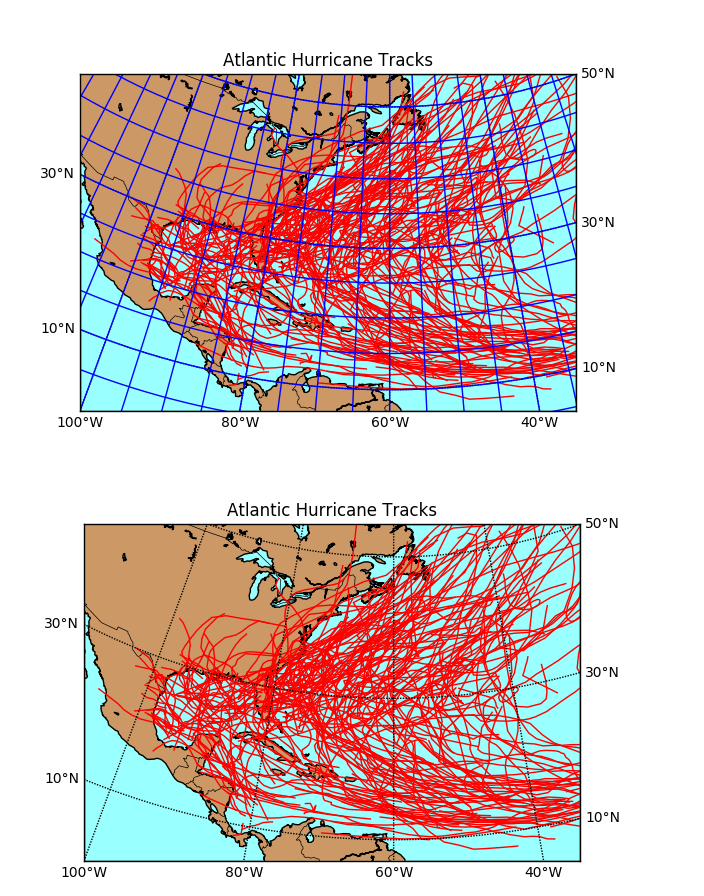
\includegraphics[scale=0.55]{Merged-Trajectory-Comparison}
\end{figure}

Consider figure (2), generated using a sample of the recorded hurricane trajectories in HURDAT2 with the visualization tool Matplotlib \cite{matplotlib}. As shown in the pair of images, region discretization organizes continuous hurricane coordinate sequences into discrete region sequences of approximately uniform size and square shape. A discretization block size of 5 is selected in HTPDM and is replicated in WARD-HTP. A block size of 5 corresponds approximately to a real-world block dimension of 500km by 500km. The block dimension size is approximate because the mapping between coordinate degrees and kilometres is imprecise, and is dependent on location in the case of longitudinal points \cite{lat-long-distance}. The approximate size of 500km is similar to the average hurricane total diameter \cite{hurricane-distances}, permitting the coarse-grain expression of hurricane trajectories without undue loss in precision.

All aspects of hurricane trajectory prediction with data mining depend on region discretization. Frequent trajectory patterns and their resulting trajectory predictions are expressed in terms of the regions where a given hurricane is expected to appear. The process of region discretization scales all hurricane coordinate trajectories downward, allowing the regionalized coordinates to be treated as a simplified coordinate system in subsequent aspects of the prediction model.

\subsection{Trajectory Matching}

The final key aspect of the hurricane trajectory prediction problem concerns accurate hurricane trajectory pattern matching. Pattern matching is a concern for hurricane trajectory prediction in two key areas. First, hurricane trajectory matching must be effectively employed when comparing a new hurricane trajectory against the table of hurricane association rules generated by the previously described variant of AprioriAll. Hurricane trajectory matching is also used when checking the correctness of a trajectory prediction. The consequent of the matched hurricane trajectory rule is compared with the actual hurricane terminal trajectory to determine prediction correctness.

\subsubsection{Rule-Fit Matching}

Pattern matching is used when evaluating the best-fit rule for hurricane prediction purposes. Similar to HTPDM, a new hurricane trajectory is passed into the hurricane prediction model proposed in this work, it is separated into two sub-trajectories: the initial trajectory $T_{i}$ and the terminal trajectory $T_{t}$. $T_{i}$ is compared against the antecedent of every interesting association rule satisfying minconf for a match. There are two dimensions that determine the best-fit rule for an incoming trajectory requiring prediction. These dimensions are matching length and rule confidence. The matching length of the initial trajectory $T_{i}$ to a rule antecedent is the longest congruent subsequence of regionalized points within the rule antecedent within $T_{i}$. Note that both $T_{i}$ and the rule antecedent sequences have been regionalized per the regionalization methodology outlined. Using the fitness function described in HTPDM \cite{major-hurricane-model}, the best-fit rule match for the incoming initial trajectory $T_{i}$ is expressed with the following formula:
\begin{eqnarray*}
Match = max( conf_{r} * (1 - e^{-matchLen_{t,r} } )\ ), r \in R
\end{eqnarray*}
Where r is a member of the set of all interesting association rules \textit{R}, t is the initial trajectory $T_{i}$, and $matchLen_{t,r}$ expresses the matching length between $T_{i}$ and the antecedent sequence of r. The match formula is meant to be maximized in order to determine the rule which most generously fits the incoming hurricane trajectory. Once the rule of best fit is determined, the rule's consequent is compared with the \textit{actual} hurricane terminal trajectory to determine if the prediction is correct.

\subsubsection{Prediction Correctness Matching}

Prediction Correctness checking is also powered by hurricane trajectory pattern matching. The consequent of the best-fit rule generated by the rule-fit matching stage constitutes the predicted terminal sequence for the incoming hurricane trajectory. The best-fit consequent is then compared against the actual terminal trajectory $T_{t}$ to determine the prediction correctness. In HTPDM and WARD-HTP, prediction correctness is considered a binary attribute: a prediction is either correct or incorrect. If the matched-rule consequent also matches the incoming hurricane terminal trajectory, the prediction is correct and the model's correctness ratio is increased accordingly.

The pattern matching for rule consequents has some differences compared to antecedent pattern matching. First, the definition of matching length is altered when considering prediction correctness. Whereas matching length for rule antecedents is the longest identical congruent subsequence of the initial trajectory, matching length for the rule consequent is the longest congruent subsequence of points within a specific distance, beginning at the start of the terminal sequence. This methodology is also based on HTPDM and is based on the following steps shown in algorithm (2). In the algorithm given, $conseq_{r}$ corresponds to the matched rule's consequent sequence and D corresponds to the minimum distance threshold necessary for prediction correctness. In HTPDM, the distance threshold corresponds to a Euclidean distance of 1.

\begin{algorithm}[H]
  \caption{Consequent Matching for Prediction Correctness}
  \label{consequent_matching}
  \begin{algorithmic}[1]
  \State{$l \gets min(|conseq_{r}|, |T_{t}|)$}
  \State{$Select\ first\ l\ points\ of\ conseq_{r}$}
  \State{$Select\ first\ l\ points\ of\ T_{t}$}
  \If{$All\ corresponding\ points\ within\ D$}
    \State{$Prediction:\ CORRECT$}
  \EndIf
  \end{algorithmic}
\end{algorithm}

The hurricane trajectory prediction model based on data mining as originally proposed in \cite{major-hurricane-model} implements all aspects of the problem domain described. Modified AprioriAll, downscaled region discretization and pattern matching with respect to association rule antecedents and consequents are respectively employed by HTPDM in order to develop an effective system for predicting future hurricane trajectories. Based on Atlantic hurricane trajectory data from 1900 to 2008, the model generates a best-case correctness ratio of 65.0\% and a worst-case ratio of 57.5\%. The training data used in the original model consists of trajectories from 1900 to 2000, with testing data supplied by trajectories from 2001 to 2008. At a high level, the model is developed and tested by following the steps below, using all implementation strategies discussed: 

\begin{enumerate}
\item Generate interesting trajectory rules from AprioriAll.
\item Determine matching rule for incoming trajectory.
\item Check if the matched rule's consequent points are sufficiently close.
\end{enumerate}

The differentiation between the model's best and worst-case hit rates is dependent on the ability of an incoming test trajectory to be matched with a trajectory association rule. As described in the pattern matching stage, the initial sub-trajectory of an incoming trajectory is compared against all interesting rules to determine a best-fit match. If no such match is found, HTPDM attempts to extrapolate a future point of the initial trajectory, using the extrapolated point as a new option for determining a rule antecedent match. When accounting for all tested trajectories, including those which were matched to a rule as a result of trajectory extrapolation or never matched with any rules, the correctness ratio was 57.5\%. Therefore, the best case correctness ratio of HTPDM is the ratio which ignores all test trajectories which did not match with any rules, resulting in a final value of 65.0\%.

Despite establishing a convincing initial start point, the best-case correctness ratio of 65.0\% may be too low for HTPDM to be considered reliable in the real-world. This is problematic for those who advocate the use of data mining in hurricane trajectory prediction as a model with only 65.0\% accuracy may not be able to deliver crucial hurricane trajectory prediction insights, particularly with respect to landfall location prediction. Both correctness ratios given must be increased in order for data mining to be considered a practical approach to predicting the trajectories of future hurricanes.

\section{Solution}

In order to increase the correctness ratio of data mining-based hurricane trajectory prediction, this work identifies and explores three opportunities for worst-case and best-case ratio refinement. The opportunities identified are the introduction of increased realism in distance calculation, the reduction of historical impact on data used, and the favourability towards recent hurricane trajectory trends. The opportunities for improvement are realized by three unique dimensions. First, the Haversine Distance Formula is employed for calculating realistic distances in spherical coordinate systems. Second, the use of weighted training data will be employed in AprioriAll to favour more recently recorded hurricane trajectories. Finally, the training data used will only constitute hurricanes from 1950 onwards to remove the risk of relying on mis-recorded historical data. The implementation of these three dimensions results in a new hurricane trajectory prediction model dubbed WARD-HTP (Weighted-Asset, Realistic-Distance Hurricane Trajectory Predictor). As shown further in this work, the combined contributions of WARD-HTP result in the desired increase to the best-case and worst-case model correctness ratios.

\subsection{Haversine Distance Formula}

The first dimension of improvement introduced by WARD-HTP is the introduction of a realistic distance formula for hurricane trajectory comparison. Two different distance measurement formulas are explored in this work for use in the correctness checking stage of the hurricane trajectory prediction model. This work compares the Euclidean distance formula against the Haversine distance formula. The Euclidean distance formula (as used in \cite{major-hurricane-model}) is designed to determine the unit distance between two N dimensional points on a plane. In HTPDM, units correspond to degrees of latitude and longitude. The Euclidean distance formula is evaluated with two dimensions, corresponding respectively to latitude and longitude values.

In contrast to the Euclidean formula, the Haversine Distance Formula is designed to determine the distance in kilometres between two latitude-longitude points over a large sphere, such as the earth's surface. Despite the fact that the earth's surface is not a perfect sphere \cite{lat-long-distance}, the Haversine Distance Formula is sufficiently accurate when used within a specific region such as the Atlantic Basin. The two formulas, denoted $D_{eucl}$ and $D_{havr}$ are defined as follows:
\begin{align*}
& (1)\ D_{eucl}(p, q) = \sqrt{(\Delta Lat)^2 + (\Delta Lon)^2}\\
& (2)\ D_{havr}(p, q) = 2R(\atantwo(\sqrt{\alpha}, \sqrt{1-\alpha}))\\
& \alpha = \sin^2(\frac{\Delta Lat}2) + \cos(p_{lat}) + \cos(q_{lat}) + \sin^2(\frac{\Delta Lon}2)
\end{align*}

% H is in RADS, Eucl in degrees
Where $\Delta Lat$ and $\Delta Lon$ respectively denote the differences in latitude and longitude between points q and p. Note that the Euclidean distance formula expresses Latitude and Longitude in degrees and minutes, while the Haversine formula expresses Latitude and Longitude exclusively in radians. In addition, whereas the Euclidean formula expresses distance in terms of units on a plane, the Haversine formula expresses distance in terms of portions of a single unit sphere. Therefore, to express distance in kilometres, the result of Haversine formula must be multiplied by R, which denotes the radius of the earth in kilometres (approximately 6371km \cite{earth-radius-kilometres}).

The euclidean distance in the discretized coordinate system corresponds to a difference in square regions approximately equal to the specified region dimension. Similar to the example outlined in section 4.2, suppose the region dimension of the discretized coordinate system is once again 5. After discretizing the coordinate system into regions of square size, a Euclidean distance of 1 between two 5-degree square regions $R_{1}$ and $R_{2}$ means that $R_{1}$ and $R_{2}$ are approximately 1 region, or 5 degrees, or 500km apart. 

When using the Euclidean formula, the distance threshold is 1. This corresponds to the distance threshold proposed in \cite{major-hurricane-model}. When the Haversine formula is employed, the maximal distance is varied from 300 to 450 km. This value corresponds to slightly less than approximately one average hurricane-diameter. Since the average hurricane diameter is between 333 and 670 km \cite{hurricane-distances}, two points are considered to be within the distance threshold if they are less than one average hurricane-diameter apart. 

The maximal distance ranges used for the Haversine formula are much less than used in the Euclidean formula. Therefore, the expected outcome of employing the Haversine formula is the production of finer-grained hurricane trajectory prediction results when compared to results generated by use of the Euclidean distance formula.

\subsection{Weighted Training Data}

The second approach to increasing trajectory prediction correctness deployed in WARD-HTP is the use of weighted training data in AprioriAll. Applying chronologically-ordered weights to recorded trajectories allows AprioriAll to favour recently produced trajectory patterns by increasing their support. While the weighting of training data results in some trajectories being counted with a support greater than 1, this effect is balanced by counting earlier recorded trajectories with a support less than 1. However, the most promising results of this work were produced when the support values for recent trajectories were increased \textit{more} than the support values for early trajectories were decreased.

In WARD-HTP, we weigh hurricane trajectories on a linearly increasing scale. This results in a tipping point \textit{T} where records before \textit{T} are underweighted and records after \textit{T} are overweighted. Depending on the weighing approach used, the combined weight of all records does not necessarily need to equal 1. The following algorithm applies further modifications to AprioriAll in order to weigh the stored hurricane records. In this algorithm, W identifies the total weighing scale to be used in the modification. For example, if W$=$3, then the final recorded hurricane trajectory in the hurricane database HDB will be counted with a support of 3. In addition, the first trajectory will be counted with a support of 3/$\lvert$HDB$\rvert$. The support modifier increases by 3/$\lvert$HDB$\rvert$ for each entry in HDB.

\begin{algorithm}[H]
  \caption{Modified AprioriAll With Weighted Support}
  \label{aprioriall_for_hurricanes}
  \begin{algorithmic}[1]
  \For{($k=1; L_{k-1} \neq \emptyset; k++)$}
    \State{$ w \gets \frac{W}{\lvert HDB \rvert}$}
    \State{$C_{k} \gets Candidates\ (Inner\ Join\ or\ Singletons)$}
    \State{$Prune\ C_{k}\ of\ infrequent\ subsequences\ $}
    \For{$sequence\ S \in HDB$}
      \State{$Increase\ c \in C_{k}\ support\ by\ w\ if\ c \in S$}
      \State{$w \gets w + \frac{W}{\lvert HDB \rvert}$}
    \EndFor
    \State{$L_{k} \gets \{c \in C_{k}|\ sup(c) \geq minsup\}$}
  \EndFor
  \State{$Frequent Trajectories \gets All(L_{k})$}
  \end{algorithmic}
\end{algorithm}

The algorithm described assumes that the HDB is ordered chronologically. This ensures that recently produced hurricane trajectory records correspond to a higher weight. Iteration through the HDB increases the current weight w by the weighting scale W divided by the size of the HDB. Therefore the final record in the HDB is guaranteed to have a weighted support exactly equal to W. Alternatively, the support weight modifier may also be changed year by year. This means that W would be divided by the number of years which the database records span, and the value of w would increase every time the records reach a new year. Though index-based weighting is shown above in algorithm (3), both year and index-based weighting strategies will be evaluated further in this work.

Assuming the input data is ordered chronologically, introducing weighted support to AprioriAll will result in higher support for patterns which occur in recent years. Recent trajectories will require less repetition to produce association rules, and higher repetition will be needed to generate frequent sequences from older data. The approach of chronologically weighted data will produce association rules that favour recent trends in hurricane trajectories. Therefore, the introduction of weighted support to AprioriAll is expected to further increase the hurricane trajectory prediction correctness ratio for current and future trajectories being tested upon. Publications such as \cite{war-mining} and \cite{cai-weighted-thesis} first introduce the use of weighted support for association rule mining. However, to the knowledge of the authors this work is the first to (1) apply weighted support to sequential data, (2) weigh individual records based on a proportional scale and (3) allow records to have a weight less than 1.

\subsection{Training Data Year Interval}

The final improvement dimension proposed in WARD-HTP is the reconsideration of 1900 to 2000 as the trajectory prediction training data interval. In its original form, HTPDM is trained on hurricane trajectory data from 1900 to 2000. However, incorporating training data from years as early as 1900 introduces a risk of skewing frequent trajectory patterns in favour of historical recording errors and climatological anomalies. While weighted support in AprioriAll helps reduce the impact of historical factors, the primitivity of early hurricane recording technology makes hurricane trajectories recorded before 1950 much less reliable than those recorded after \cite{hurricane-recording-history}.

The hurricane trajectory prediction model proposed in this work relies on test data exclusively from trajectories recorded between the years 1950 and 2000. The motivation being selecting this specific year interval is the attempted reduction of historical factors in the generation of frequent trajectory patterns (and subsequent interesting trajectory association rules). Paired with the Haversine Distance Formula and weighted AprioriAll approaches, tweaking the training data year interval is expected to result in an additional increase of the model correctness ratio. Additionally, association rules generated by training data from 1950 and onwards are expected to be more reliable as the influence of historical factors will be removed.

\section{Experimental Setup}

In its fully implemented form, WARD-HTP was run against various input parameters to determine an optimal configuration. WARD-HTP was evaluated against varying distance formula styles, weighted training data approaches (including the absence of weighted data), and training data year intervals. Evaluation of WARD-HTP was conducted on an eight-core Intel(R) i7-4720 processor at 3.35GHz, with 8 GB of memory using a Python implementation. The training and testing data was supplied from Hurricane DATabase 2 (HURDAT2), which is maintained by the National Oceanic and Atmospheric Administration \cite{HURDAT2-original}.

Apart from the three dimensions of improvement outlined, one of the key differences between HTPDM and WARD-HTP is that WARD-HTP does not attempt to extrapolate points for hurricane trajectories with which no rules were successfully matched. Therefore, results shown from WARD-HTP capture the correctness ratio when considering all test trajectories, and the correctness ratio when exclusively considering trajectory with which a rule was immediately successfully matched. Rule-match extrapolation was omitted from WARD-HTP due to the nature of the trajectories recorded in HURDAT2.

\begin{figure}[htp]
\caption{Non-Matchable Hurricane Trajectory Paths}
\centering
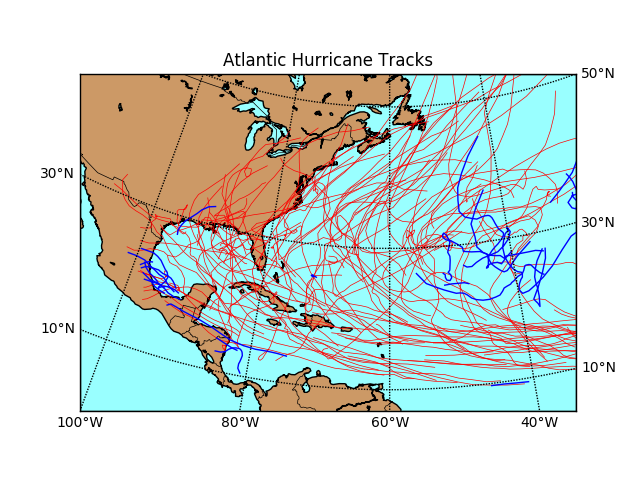
\includegraphics[scale=0.6]{Rule-Miss-Diagram}
\end{figure}

Figure (3) illustrates the characteristics of trajectories which were not able to match with any interesting rules. The particular diagram was generated from training data ranging from 1950 to 2000, and testing data from 2001 to 2015. Red trajectories represent a subset of the training data, while blue trajectories are those which did not match with any association rules. It is visually clear to see that non-matching trajectories were highly dissimilar from training data trajectories. As a result, no amount of point extrapolation would be able to result in a reliable terminal trajectory prediction. Some of the non-matching trajectories appear to align with training trajectories, but are moving in an opposite direction. Therefore, any points that matched such trajectories would also not provide a reliable result.

\section{Experimental Results}

This section documents the experimental results of all improvement dimensions proposed in WARD-HTP. The respective dimensions of Haversine Distance, Weighted Training Data and Training Data Year Interval of 1950-2000 contribute iteratively to a total growth in best-case correctness ratio of 10.0\% when compared to HTPDM, for a total of 75.0\%. Whereas the worst-case correctness ratio (ratio accounting for rule-miss incidents) of HTPDM was 57.5\%, the worst-case correctness ratio of WARD-HTP was 72.58\% when configured in the same manner that generated the best-case result of 75.0\%. 

The worst-case to best-case difference in HTPDM is 7.5\%, whereas the difference between the two cases in WARD-HTP is 2.44\%. This results in a difference decrease of 5.08\%. Not only is the difference in ratios reduced when using WARD-HTP, the best and worse case ratios are also increased, by 10.0\% and 5.08\% respectively.

\subsection{Haversine Distance Formula}
\begin{figure*}[!bp]
\centering
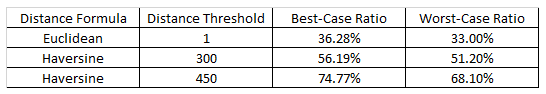
\includegraphics[scale=1.0]{Distance-Formula-Results}
\caption{Results of Different Distance Formulas}
\end{figure*}

The Distance Formula section of the experiments in this work compare the Euclidean Distance approach as seen in HTPDM against two separate Haversine Distance approaches. The first approach imposes a distance threshold \textit{D} of 300km while the second sets \textit{D} to 450km. 300km was selected as a sample value for testing the Haversine formula, while 450km was selected as a value slightly less than the approximate average hurricane diameter as discussed in section 4-B. 

Aside from differences in the distance approaches, all other variables in this experiment are held constant. The model was trained on trajectories recorded between 1950 and 2000 and tested on trajectories recorded between 2001 and 2015. The parameters of AprioriAll were set to minsup$=$3.75\% (28.3125) and minconf$=$0.25. The training data in AprioriAll was unweighted (weighing scale$=$1), and rule-miss extrapolation was disabled as previous discussed.

As shown in figure (4), the Euclidean distance option resulted in much lower correctness ratios than both the 300km and 450km Haversine approaches. The Haversine Distance approach with \textit{D} set to 450km produces the highest best and worse-case correctness ratios. While the difference between ratios is smallest when using the Euclidean distance formula, the overall increase in both ratios makes the Haversine distance at \textit{D}$=$450km the optimal selection. The distance threshold of 450km introduces more flexibility into which predictions count as correct. The increase in flexibility is permissible as 450km still corresponds to a size smaller than the approximate average hurricane diameter. The results of this section show that using the Haversine Distance formula with a threshold of 450km is the ideal approach to evaluating distance when predicting hurricane trajectories with data mining.

\subsection{Weighted Training Data}

\begin{figure*}[!bp]
\centering
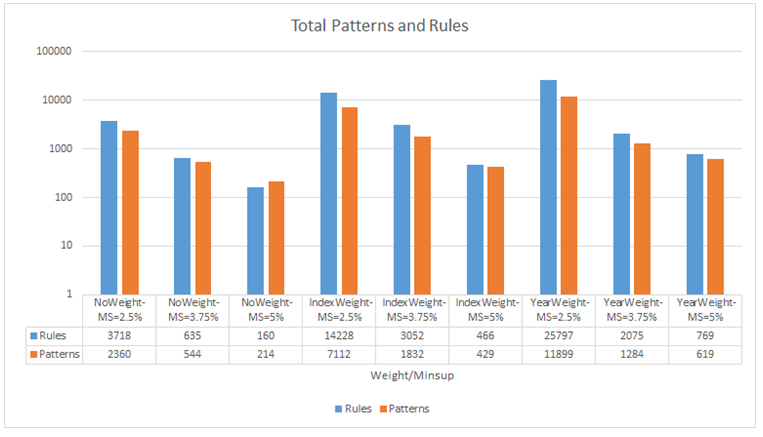
\includegraphics[scale=0.8]{Patterns-Rules-Weight-Metrics}
\caption{Minsup and Weighing Strategies Against Patterns and Rules}
\end{figure*}

In this section of the evaluation against WARD-HTP, multiple complete executions of the model, from AprioriAll to the correctness ratio analysis, are completed. Each execution of WARD-HTP is performed on a unique pairing of minimum support and training data weighting strategy with the weighing scale W set to 2.5. The weighting strategy options also includes the absence of any weighting strategy. Apart from the minimum support and the weighting strategy, all other parameters of the model are held constant.

Three different weighting strategies are evaluated in this experiment. First, the absence of data weighing is explored. Next, weighting on an annual scale is considered. In this strategy, the value of w increases by W divided by the total number of years in the data Y (in the case where training data is supplied from 1950 to 2000, Y$=$50). The third strategy employed is the index-weight strategy, where the weight is updated at each HDB entry.

Various values of minimum support are also explored in this series of evaluations. Minimum support values corresponding to 2.5\%, 3.75\% and 5\% of the number of training data trajectories are paired against the three weighing strategies discussed above. While a higher minimum support will generate fewer interesting trajectory association rules, the rules generated may be more reliable for future predictions.

In figures (5) and (6), the number of frequent trajectories and trajectory association rules generated is compared alongside the best and worse case hit rates produced for given pairings of minsup and the weighing strategy. Note that the minconf value is held at 0.25 for all experiments, along with the training data of 1950-2000 from HURDAT2, testing data from 2001-2015, and distance formula set to Haversine Distance with a threshold of 450.

The maximal best-case hit rate for WARD-HTP was generated with a year-weighted strategy and minimum support set to 2.5\%, corresponding to 18.875 when used with data from 1950 to 2000. The resulting hit rate was 75.0\%, with a worst-case of 72.58\%. Note that a minimum support of 5\% with index-based weighting generated a very slightly higher best-case hit rate at 75.22\%, though with a lower worst-case ratio of 67.33\%. We select 75\% as the optimal generated data point because a .22\% decrease in best-case hit rate is certainly a ``fair trade'' for a 5.25\% increase in worst-case hit rate. 

The year-based and index-based weighting strategies generated identical model results at minsup$=$2.5\%. We select the year-based weighting strategy as the optimal approach due to the fact that the year-based strategy evenly counts trajectory records with respect to time. In the year-based strategy, all records from the most recent year are counted at the maximum weight scale, whereas the index-based strategy only counts one record at the maximum. While the two weighting strategies resulted in identical results in this scenario, the year-based strategy is preferred as it closely couples the increase in support weight to real-world historical hurricane trajectory trends.

\begin{figure*}[!tp]
\centering
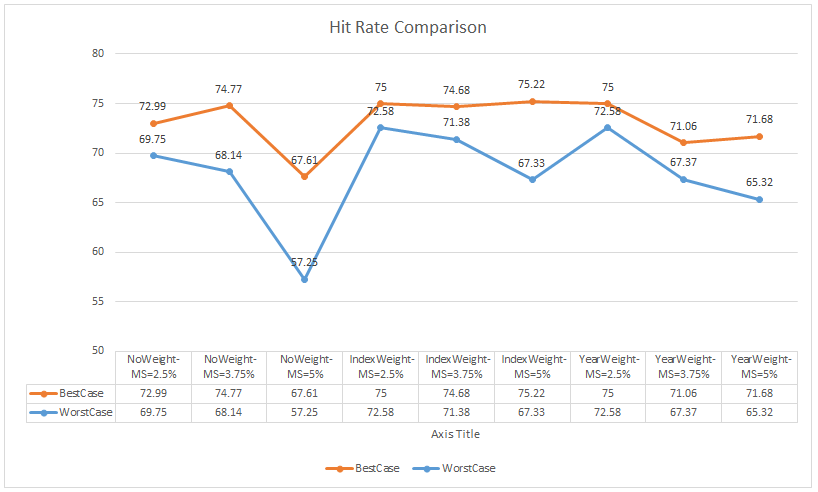
\includegraphics[scale=0.8]{Hit-Rate-Weight-Metrics}
\caption{Minsup and Weighing Strategies Against Correctness Ratios}
\end{figure*}

\subsection{Training Data Year Interval}

The final component of the evaluation undertaken in this work compares the correctness ratios generated by various training and testing data intervals. Training data from 1900 to 2000 and 1950 to 2000 is used against testing data from 2001 to 2008 and 2001 to 2015. All other variables are held constant with minsup$=$2.5\%, weighting strategy set to yearly and the distance formula set to Haversine with \textit{D}$=$450. Note that the data ranges used by HTPDM were 1900-2000 for training data and 2001-2008 for test data.

\begin{figure}[htp]
\centering
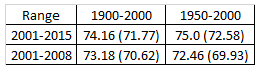
\includegraphics[scale=1.0]{Year-Interval-Metrics}
\caption{Year Interval Options Against Correctness Ratios}
\end{figure}

Figure (7) shows the correctness ratios generated by all possible training data and testing data pairings. Note that ratios in brackets denote the worse-case ratio while ratios outside of brackets refer to the best-case. Between all possible options, we find that the training data interval of 1950-2000 results in the best correctness ratios for testing data from 2001-2015 when applying all other parameters we deemed optimal throughout the previous results of this work. Regardless of correctness ratio, 2001-2015 should always be selected as the test data interval to encourage analysis against more recent hurricane patterns. The results show that no training-data/testing-data pairing was able to generate correctness ratios higher than the ones generated by training the model with data from 1950 to 2000, and testing it on data as recently recorded as 2015.

\section{Conclusions and Future Work} % what we found:

This work proposed a new model named the Weighted-Asset, Realistic-Distance Hurricane Trajectory Predictor (WARD-HTP) for improving the accuracy of existing data mining approaches to hurricane trajectory prediction. An AprioriAll-based hurricane trajectory prediction model similar to \cite{major-hurricane-model} was developed to demonstrate the unique contributions of WARD-HTP. There are three such contributions brought forth in the development and implementation of the model proposed. These contributions are the use of training data from 1950 to 2000, the use of weighted training data, or weighted assets (WA), and the use of the Haversine Distance Formula for realistic distance (RD). The three contributions combined form WARD-HTP and produce a hurricane trajectory prediction correctness ratio of exactly 75.0\%, which is 10\% higher than the current state-of-the-art. When accounting for trajectories which were not able to match with any association rules, the correctness ratio of WARD-HTP is 72.58\%, which is still 5.08\% higher than the worst case state-of-the-art ratio of 57.5\% as seen in \cite{major-hurricane-model}.

There are multiple areas to explore in the hurricane trajectory prediction problem space with respect to future work. Experiments in this work show that all datasets contain a subset of trajectories for which no association rule could be matched. While \cite{major-hurricane-model} proposed an extrapolation method to recover from rule-miss incidents, more work must be completed to reduce the number of non-matchable trajectories. Many of the mismatched trajectories are outliers with very little conformance to existing hurricane trajectories as seen in figure (3). Additionally, more experiments will be run on different inputs including training data from other regions such as the Pacific region. Further approaches to increasing the correctness ratio of WARD-HTP will also be investigated. This includes the investigation of alternative methods for defining training data weight.

\begin{thebibliography}{1}
\bibitem{hurricane-cost} Pielke Jr, Roger A., et al. Normalized hurricane damage in the United States: 1900–2005. Natural Hazards Review 9.1 (2008): 29-42
\bibitem{hurricane-cost-non-financial} F. F. Townsend, The Federal Response to Hurricane Katrina: Lessons Learned, United States Federal Government, Washington, DC, USA, 2006
\bibitem{data mining-def} S. Sumathi and S. N. Sivanandam, Introduction to Dataming and its Applications: Springer Publishing 2006, ISBN: 978-3-540-34350-9
\bibitem{major-hurricane-model} Dong, X and C. Pi, D. (2013). Novel method for hurricane trajectory prediction based on data mining. Natural Hazards and Earth System Sciences. 13. 3211-3220. 10.5194/nhess-13-3211-2013. 
\bibitem{HURDAT2-original} C. Landsea, J. Franklin and J. Beven (2015) The revised Atlantic hurricane database (HURDAT2). National Oceanic and Atmospheric Administration
\bibitem{AprioriAll-original} R. Agrawal and R. Srikant, Mining sequential patterns, Proceedings of the Eleventh International Conference on Data Engineering, Taipei, 1995, pp. 3-14.
doi: 10.1109/ICDE.1995.380415
\bibitem{hurricane-intensity-1} Y. Su, S. Chelluboina, M. Hahsler and M. H. Dunham, A New Data Mining Model for Hurricane Intensity Prediction, 2010 IEEE International Conference on Data Mining Workshops, Sydney, NSW, 2010, pp. 98-105
doi: 10.1109/ICDMW.2010.158
\bibitem{hurricane-intensity-2} R. Yang, J. Tang and D. Sun (2011), Association Rule Mining Application for Atlantic Tropical Cyclone Intensity Changes, American Meteorological Society. doi: 10.1175/WAF-D-10-05029.1
\bibitem{hurricane-forecasting-1} Rozanova, Olga S., Jui-Ling Yu, and Chin-Kun Hu. Typhoon eye trajectory based on a mathematical model: Comparing with observational data. Nonlinear Analysis: Real World Applications 11.3 (2010): 1847-1861.
\bibitem{hurricane-forecasting-2} Chandan Roy and Rita Kovordanyi, Tropical cyclone track forecasting techniques: A review, 2012, Atmospheric research, (104-105), 40-69. doi: 10.1016/j.atmosres.2011.09.012.
\bibitem{typhoon-clustering} Kim, Hyeong-Seog, et al. Pattern classification of typhoon tracks using the fuzzy c-means clustering method. Journal of Climate 24.2 (2011): 488-508.
\bibitem{matplotlib} J. D. Hunter, Matplotlib: A 2D Graphics Environment, in Computing in Science and Engineering, vol. 9, no. 3, pp. 90-95, May-June 2007.
doi: 10.1109/MCSE.2007.55
\bibitem{lat-long-distance} Menno-Jan, K. (2013). Map use: reading, analysis, interpretation: by Kimberling, AJ, Buckley, AR, Muehrcke, PC and Muehrcke, JO, Redlands, California, ESRI Press Academic, 2012. ISBN 978-1-589-48279-1 Seventh edition.
\bibitem{hurricane-distances} D. Brown. (2013) Forecast Verification: Quantifying Forecast Uncertainty. National Hurricane Conference: Hurricane Readiness for Coastal Communities
\bibitem{earth-radius-kilometres} Chambat, F., and Valette, B. (2001). Mean radius, mass, and inertia for reference Earth models. Physics of the Earth and Planetary Interiors, 124(3), 237-253.
\bibitem{war-mining} W. Wang, J. Yang and P. Yu Efficient  mining of  weighted association rules (WAR), Proc. of the ACM SIGKDD Conf. on Knowledge Discovery and Data Mining, 270-274, 2000.
\bibitem{cai-weighted-thesis} Cai, Chun Hing, Ada Wai-Chee Fu, C. H. Cheng, and W. W. Kwong. Mining association rules with weighted items. In Database Engineering and Applications Symposium, 1998. Proceedings. IDEAS'98. International, pp. 68-77. IEEE, 1998.
\bibitem{hurricane-recording-history} Landsea, C. W., Vecchi, G. A., Bengtsson, L., and Knutson, T. R. (2010). Impact of duration thresholds on Atlantic tropical cyclone counts. Journal of Climate, 23(10), 2508-2519.

\end{thebibliography}

\end{document}